\chapter{Software Development}
\label{chap:Software Development}

The development of two core project deliverables will be discussed:

\begin{enumerate}
\item Functional configuration, control and logging platform.
\item Reliable embedded system control system and motor driver communication protocol. 
\end{enumerate}

The following software development environments were considered: C/C++ (Qt), Python, Processing (dedicated graphic programming), and Matlab (serial toolbox). 

The Qt C/C++ GUI development environment was chosen for the following primary reasons:

\begin{itemize}
\item Low over-head programming language.
\item Open source software.
\item Low level computer hardware access results in near real-time serial packet processing and accurate timing.
\item Compatibility with C packed struct packet encoding and decoding code (as developed in \cref{sec:Packet Transmission}).
\end{itemize}

The design, operation and commissioning of the software system will be covered in detail. 

\section{RTOS Communication Protocol}

Ideally FreeRTOS tasks should operate with as much isolation as possible, with each task performing a specific function with different priority levels. In the case of a communication protocol, the overall task is inherently sequential so this leads to FreeRTOS being used in a sequential way with all tasks operating at real-time priority level. 

FreeRTOS was chosen because of the following benefits:

\begin{enumerate}
\item Segmentation of code into specific tasks provides readable code for future users.
\item FreeRTOS task configuration provides a framework for future embedded robotic control systems as well as easily reconfigurable code.
\item Semaphores and queues lend themselves to sequential reception and processing of packets at predefined intervals very well.
\item Isolation of tasks provides easy debugging of communication issues.
\end{enumerate}

\subsection{Heartbeat Task}
The \textit{Heartbeat} task's primary function is to synchronise the communication protocol. It is the only task running with a 5 ms non-blocking delay. Every 5 ms it completes the following functions:

\begin{enumerate}
\item Compiles a read command packet for current, position and velocity.
\item Appends these three packets to the two motor driver transmit queues. 
\item Gives a binary semaphore to the motor 1 and motor 2 transmit tasks.
\item Starts a 5 ms non-blocking delay to allow the two motor transmit tasks to complete their transmission and for the motor driver replies to be received and decoded.
\item Gives a binary semaphore to the PC transmit task to compile and send the newly received motor data for logging.
\end{enumerate}

\subsection{PC TX Task}
The \textit{TXPC} task is used purely for logging of data over serial on the Baleka C++ application, as seen in \cref{chap:Graphic User Interface}. 

Data is received in a queue from both the motor \textit{RXMotor1} and \textit{RXMotor2} tasks as well as the \textit{Controller} task which is compiled into a packet along with status bits indicating various events and conditions. 

Status bits in the packet indicate to the PC logging software whether specific data has been successfully received by the \textit{PCTX} task in the queue. A CRC check is added for transmission based error detection. 

The task is run every $5\ ms$ once the motor data has been requested, received and processed, and the \textit{Controller} task has instructed the motor drivers to perform a specific command. 

\subsection{PC RX Task}
The \textit{RXPC} task is the only task that is required to perform non-synchronous reception of packets. The DMA reception is initialised and then the task waits until the full PC packet has been received. The RX complete interrupt handler then gives the \textit{PCRX} task a semaphore to continue decoding of the data. The use of non-blocking DMA UART reception and semaphores ensures other tasks are able to run during the reception process.

The \textit{RXPC} task checks how much data has been received before searching for the start-bytes of the packet. Once a valid packet has been found it is copied to a packed struct  and the CRC is calculated and compared to the CRC member of the struct. If it is valid then the \textit{RX\_DATA\_VALID} flag is set, this indicates to other tasks that they can safely use the packet data received. 

Every packet has an op-code that indicates what data is present in the packet. A switch statement is used to process the data appropriately and perform the necessary functions. These functions range from configuring the motor drivers, killing the drivers, calibrating motor positions and triggering various on-board events such as jumping and leg trajectories. All these functions operate by setting flags or compiling packets to be sent to the necessary queues for transmission.

An example of the packet processing code can be seen in \cref{listing:PC RX packet processing}.

\subsection{TX Motor Task}
The \textit{TXMotor} task functions as an interface between the rest of the tasks and the motor driver. The task is periodically run when a semaphore is received.

When the task starts a DMA reception from the motor drivers is initialised, which will only be halted once control is handed over to the \textit{RXMotor} task. 

Every time the task runs, at least three command packets are sent to the motor driver from the \textit{TransmitMQ} queue. This queue is filled by the \textit{Heartbeat} task which synchronises all communication protocol tasks. The three command packets request current, position, and velocity data from the motor drivers which is processed by the \textit{RXMotor} task and used in the control loop every $5\ ms$. 

The queue runs in a loop until transmission is complete, with a number of timing conditions being completed to ensure that a reply is received from the motor driver before the next request is transmitted - if this is not done properly then data can be lost. 

The other three queues are used for current commands, position commands, and for general motor driver management commands such as changing gain sets or initialising the motors. An important task for the general driver management queue, \textit{CommandMQueue}, is to disable the motor drivers when position and/or current limits are reached.

\subsection{RX Motor Task}
The \textit{RXMotor} task is used to process data received from the motor driver in a reply to a command. The task waits to receive a semaphore from the \textit{TXMotor} task, after which the DMA reception is halted. 

The task then begins processing the data by:

\begin{enumerate}
\item checking how much data has been received,
\item  searching the buffer and finding the index of all start bytes,
\item finding unique user programmable op-codes based on location of start bytes,
\item using a switch statement to appropriately decode data using a packed struct based on the op-code,
\item and adding this data to a buffer before moving on to the next start byte index for processing.
\end{enumerate}

This data buffer is then sent to the \textit{Controller} and \textit{TXPC} task queue before waiting for a semaphore to be received again.

\subsection{Controller Task}

The controller task's core function is to reliably implement the control loop design seen in \cref{fig:virtual-model-impedance-loop} and developed in \cref{chap:Controller Development}. This means the controller task runs at a consistent $200\ Hz$ frequency.

The control loop waits for new data to be received from each motor on a queue from the \textit{RXMotor} task - this is expected to happen every $5\ ms$. If an error occurs or the data received from the drivers is invalid then the control loop will not run for safety. 

Once the data has been received, if a valid \textit{RXPC} packet is available it is checked for virtual model configuration data which is then used to set up the spring-damper model.

A \textit{TRIGGER} flag and \textit{START} flag are both checked before functions are run or the controller is allowed to operate. The \textit{TRIGGER} flag is used to start jump and trajectory sequences.

Multiple calculations are performed to implement a control model:

\begin{enumerate}
\item Cumulative integral error term.
\item Jacobian mapping for velocity and position.
\item Spring-damper force vector which is mapped using to motor torques using Jacobian.
\item Torque current command mapping using torque constant as derived in \cref{sec:Motor Model Calculations}.
\end{enumerate}

If there are invalid kinematic or current set-points a kill function is implemented that both stops the control loop from operating and kills the motor driver bridge.

If a current command is successfully calculated, a motor driver command is compiled and sent to the \textit{TXMotor} task queue.

\subsection{FreeRTOS Timing}

The default 1000 Hz tick rate was overridden with a tick rate of 5000 Hz to enable more fine tuned packet timing and delays. The timing configuration can be seen in \cref{listing:FreeRTOS timing}. 

In order to achieve a control loop rate of 200 Hz, a sampling time of 5 ms or 25 ticks was used.

\begin{figure}
\centering
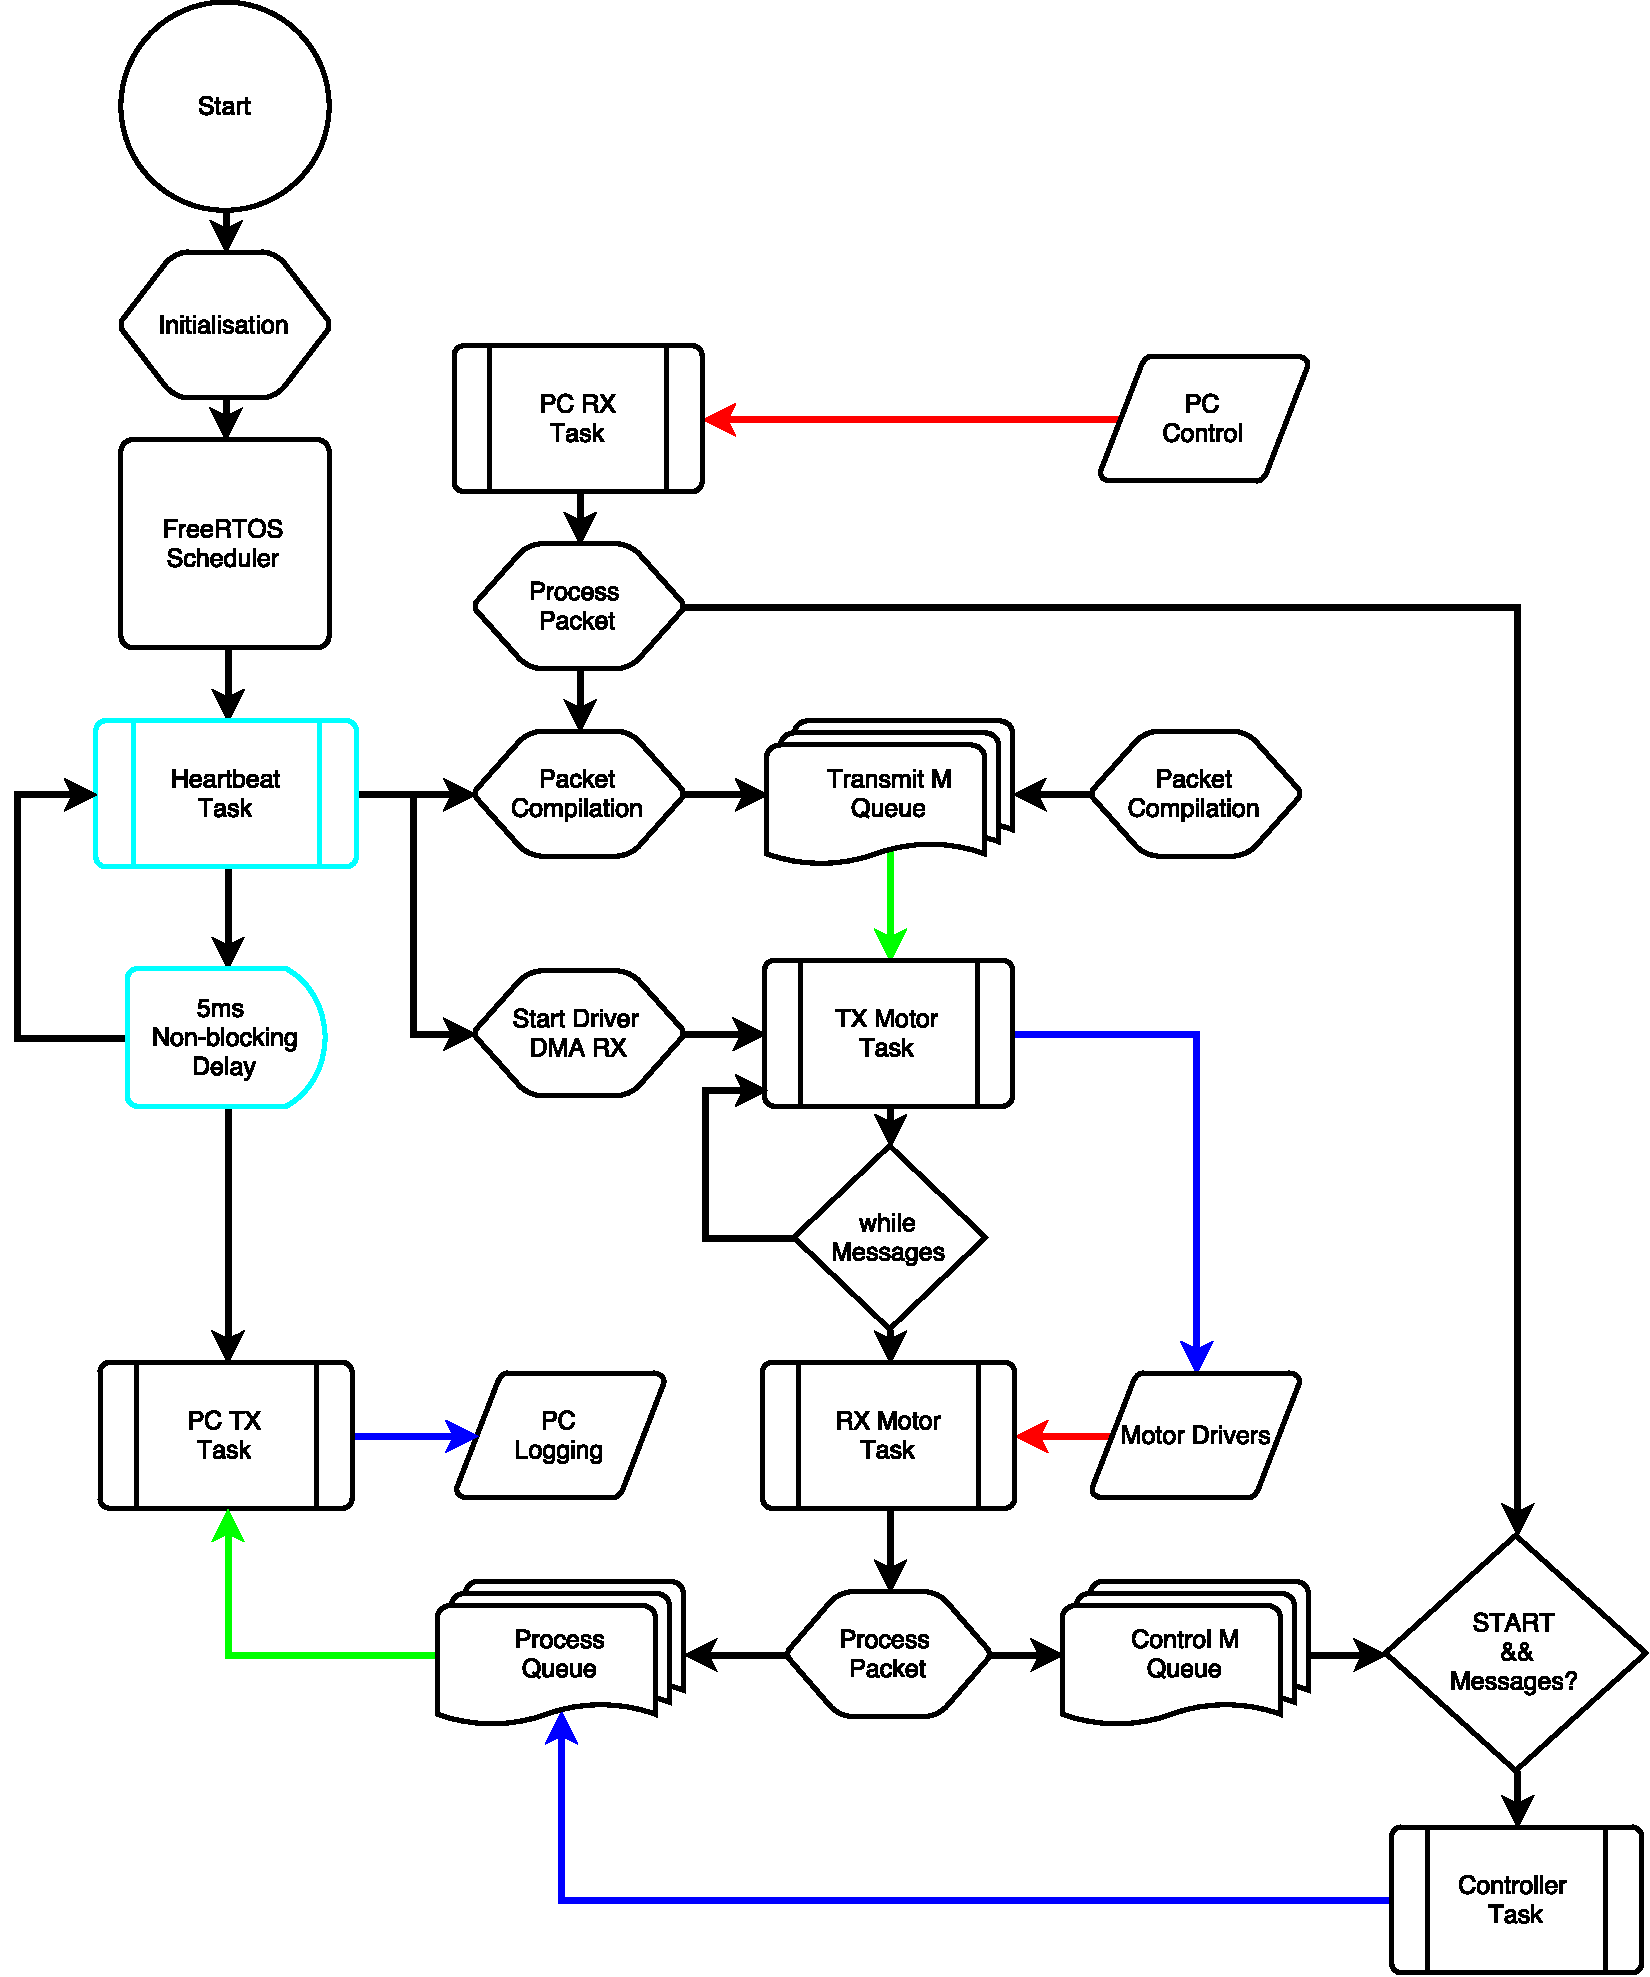
\includegraphics[width=1\textwidth]{images/comms/communication-flow-diagram.pdf} 
\caption{FreeRTOS communication protocol flow diagram.}
\label{fig:FreeRTOS communication protocol flow diagram.}
\end{figure}

\section{Packet Transmission}
\label{sec:Packet Transmission}

\subsection{Structuring}
\label{sec:structuring}

Usually when a C compiler stores data in memory it does so in a manner that optimizes memory access speed. In the case of a struct this isn't intuitively in successive memory addresses, but with padding.

Packets are compiled and transferred in bytes, the smallest variable size on any architecture apart from bit fields. A simple and elegant solution to packet structuring and decoding is to use a struct where the individual bytes are consecutive and byte aligned, much like an array, but with the benefit of accessing by struct member too.

This method has a few major benefits:
\begin{itemize}
\item To decode packets the data can be copied from a receive buffer directly over a struct and each of the struct members will contain the appropriate "decoded" data.
\item To structure and compile a packet, all the relevant data can be assigned to a struct member and then when the packet is ready to be transmitted it is as simple as passing a pointer to the first value of the struct along with the packet length.
\item The CRC check can be performed on a sequence of struct members with the guarantee that all members are consecutive and byte aligned.
\item The packet length is the size of the struct!
\end{itemize}

The way to ensure that bytes are consecutive and byte aligned is to use the $\_\_$attribute$\_\_$((packed)) C compiler type attribute. This is a compile time flag that forces the struct to be byte aligned with no padding. An example of a packed struct from the embedded software can be seen in \cref{listing:packed-packet} in \cref{app:Communication Protocol Code}.

\subsection{Integrity Checking}

A Cyclic Redundancy Check was implemented for all communication. Polynomial division is performed on the data contents of the packet, this results in a remainder that constitutes the CRC that is appended to the packet. If this CRC does not match the calculated CRC on the receiver side then measures are taken to deal with the corrupt packet. 

The CRC ensures the communication system is robust to interference and corruption, which can come from a number of sources:

\begin{itemize}
\item 3 phase alternating current flowing through motor phase wires.
\item Motor EMF generated.
\item RTOS and embedded system errors due to synchronisation.
\end{itemize}

Two CRC protocols were used. The CRC calculation function developed by James Gowans in December 2012 was customized to work with the motor driver two byte CRC protocol.

The iNemo and PC packets used the CRC-16/CCITT-FALSE protocol and the motor drivers are hard-coded to use the XMODEM protocol, with the configuration seen in \cref{tbl:CRC protocol configuration} and originally found in \cite{gregcook2016}.

In order to reduce CPU time used for CRC calculations, two CRC lookup tables are generated before the RTOS scheduler takes control.

\begin{table}[]
\centerline{
\begin{tabular}{lllllllll}
\textbf{Device}       & \textbf{Protocol} & \textbf{Width} & \textbf{Polynomial} & \textbf{Init} & \textbf{Refin} & \textbf{Refout} & \textbf{XORout} & \textbf{Check} \\
\textbf{iNemo/PC}     & CCITT-FALSE       & 16             & 0x1021              & 0xffff        & FALSE          & FALSE           & 0x0000          & 0x29b1         \\
\textbf{Motor Driver} & XMODEM            & 16             & 0x1021              & 0x0000        & FALSE          & FALSE           & 0x0000          & 0x31c3        
\end{tabular}
}
\caption{CRC protocol configuration.}
\label{tbl:CRC protocol configuration}
\end{table}

\subsection{Compilation}

\subsubsection{Motor Driver Packet}

A function was created to compile motor driver command packets based on the AMC motor driver packet protocol. The \textit{BaseCommandCompile} function prototype can be seen in \cref{listing:Motor packet compilation function}. 

All motor driver packets either request data from a memory address or contain data to be written to a memory address. The command bits \textit{ComBits} of the function are written to the packet, where 0x02 tells the motor driver to set data and 0x01 tells the motor driver to read data. \textit{INDOFF1} and \textit{INDOFF2} indicate the motor controller address and offset for reading or writing of data. 

The \textit{SeqBits} are a unique sequence of 4 bits that function as an ID for the packet - the motor driver will reply with the same ID to indicate which command it is responding to. The response sequence bits are then used as an op-code for the packet processing switch statement used in the \textit{RXMotor} RTOS task.

Some of the function inputs set up the structuring of the packets and identify the packets within the embedded system. \textit{DATA} is a pointer to the data to be written to the address, \textit{LEN} indicates how many bytes of data must be read from the motor driver address and \textit{SNIP} is a parameter that is a workaround for proper packet compilation indicating how many bytes must be removed from the packet if the packet is for requesting data rather than writing data.

The final function input, \textit{n}, is an index for the packet. This is an index for the array of structs that is used to compile the packets. This way when a packet command is to be sent to a function on one of the RTOS queues, just the index can be sent. 

An example of an array of structs can be seen in \cref{listing:Motor packet array of structs} and an example usage of the \textit{BaseCommandCompile} function can be seen in \cref{listing:Motor packet compilation example}.

All of the parameters, op-codes and other information relating to motor command packet encoding can be found in \cref{tbl:motor-driver-protocol} in \cref{chap:Motor Driver Command Protocol}.

\begin{listing}[]
\begin{minted}[
linenos,
bgcolor=smokyblack]{c}
void BaseCommandCompile(uint8_t n, uint8_t SeqBits, uint8_t ComBits, 
uint8_t INDOFF1, uint8_t INDOFF2, uint8_t *DATA, 
uint8_t LEN, uint8_t SNIP);
\end{minted}
\caption{Motor packet compilation function.}
\label{listing:Motor packet compilation function}
\end{listing}

\subsubsection{PC Packet}

The structure of the packets both received and transmitted by the PC can be seen in \cref{fig:pc-rx-packet} and \cref{fig:pc-tx-packet} respectively.

The typical start and stop byte (one) were replaced with start and stop bytes (two), being \textit{~[} and \textit{]~} respectively. This removed the need to search for and remove any start or stop byte in the packet data before transmitting. The chance of there being a series of two start or stop bytes in the data is $1$ in $16\times 16\times 16\times 16 = 65536$. 

In \cref{fig:packet-timing} the transmission duty cycle for packets transmitted from the embedded system to the PC, the larger of the two packets, is approximately $20 \%$ - this leaves plenty of time for additional data to be transmitted. The PC TX packet is 75 bytes and the PC RX packet is 59 bytes. As additional data is appended to the packets via the packed struct, the protocol allows for quickly reconfiguring transmission and reception processes to accommodate this extra data for logging and live plotting. 

The status bit field of the packet allows individual bits to be used as variables - this is a special C variable type that is useful for creating a sort of binary flag in the packet. 

The trigger bits of the \textit{PC TX} packet allows various events and sequences to be started in the embedded system control loop.

\begin{figure}
\centering
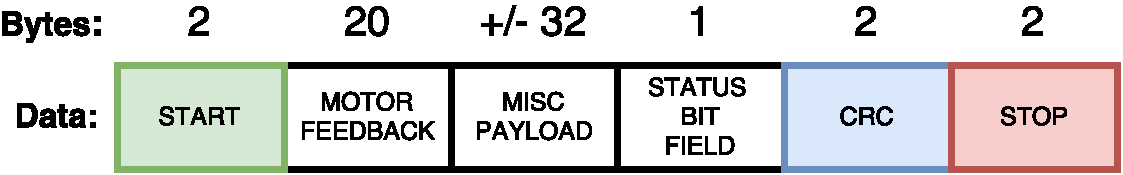
\includegraphics[clip, trim=0cm 0cm 0cm 0cm, page = 1, width=1\textwidth]{images/comms/pc-rx-packet.pdf} 
\caption{PC RX packet structure.}
\label{fig:pc-rx-packet}
\end{figure}

\begin{figure}
\centering
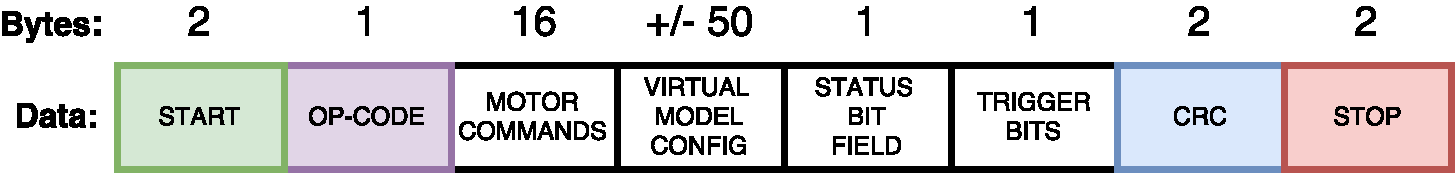
\includegraphics[clip, trim=0cm 0cm 0cm 0cm, page = 1, width=1\textwidth]{images/comms/pc-tx-packet.pdf} 
\caption{PC TX packet structure.}
\label{fig:pc-tx-packet}
\end{figure}

\section{Peripheral Configuration}

A basic peripheral configuration diagram can be seen in \cref{fig:microcontroller-peripheral-config} showing which UART and GPIO ports are routed to which pins.

\begin{figure}
\centering
\includegraphics[clip, trim=1cm 7cm 1cm 7cm, page = 2, width=0.8\textwidth]{pdfs/BalekaSTMConfig.pdf} 
\caption{STM32F4 microcontroller peripheral configuration.}
\label{fig:microcontroller-peripheral-config}
\end{figure}

\subsection{Protocol}

A number of serial protocols were used in the communication system. To reduce noise interference from motor EMI the RS-485 protocol was used. RS-485 uses differential signalling with a $200\ mV$ binary threshold. This protocol is designed for long distance low noise data transmission at data rates up to $10\ MBits/s$ at short to medium range. 

The VD30 and VD485 RS-485 driver ICs were used to couple the TTL serial logic of the microcontroller to the RS-485 transmission lines. A RS-485 to TTL serial USB converter was used to interface with the PC. The iNemo microcontroller was directly connected via TTL level serial to the microcontroller. The communication protocol configuration can be seen in \cref{fig:uart-communication}.

\begin{figure}
\centering
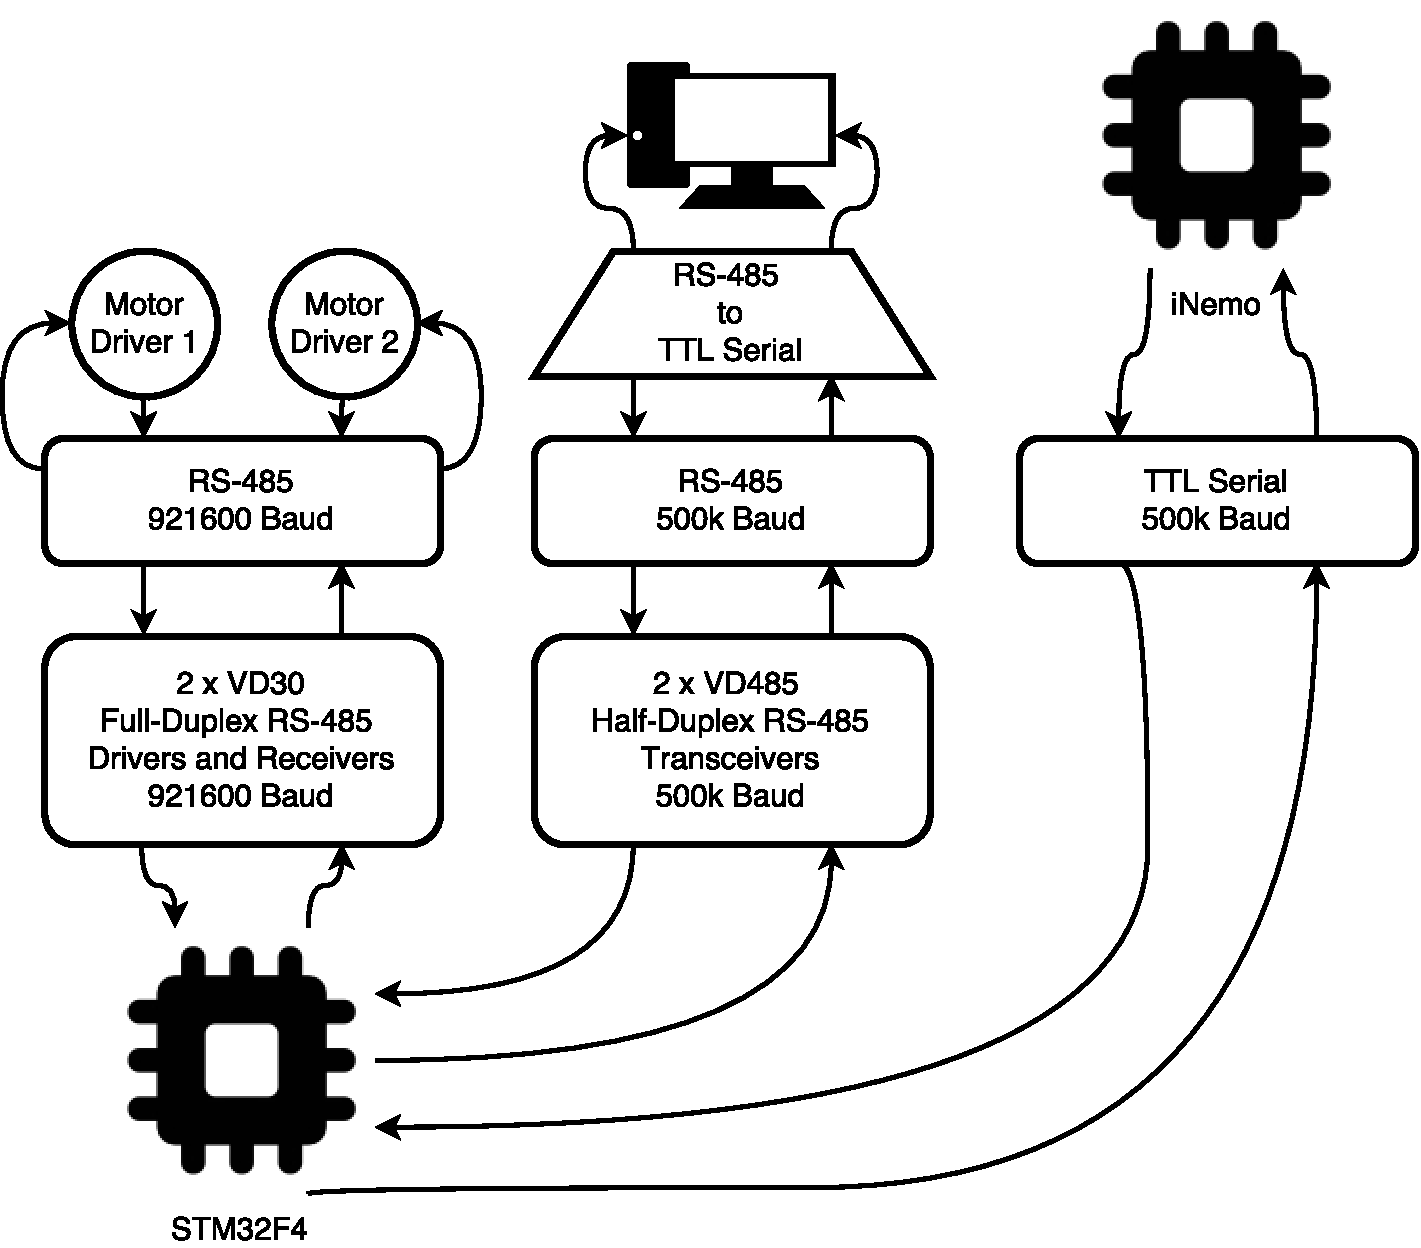
\includegraphics[width=0.8\textwidth]{images/comms/uart-communication.pdf} 
\caption{STM32F4 UART Serial Protocol.}
\label{fig:uart-communication}
\end{figure}

\subsection{Data Rates}

Two data rates were selected for the motor driver interface, and the iNemo and PC interface. 

The maximum communication speed of the motor controllers is 921600 baud over RS-485. Due to the high speed control loop frequency, and in order to achieve the high density packet transmission and reception as seen in \cref{fig:packet-timing}, the 921600 baud rate was selected.

In \cref{fig:packet-timing} the motor 1, M1, command and reply sequence can be seen. Every time a command is sent the corresponding reply has to be received before the next command can be sent. This is an on-board motor driver problem, when commands are sent before the previous reply the motor driver fails to perform the command. This bottle neck greatly reduced possible control loop frequency. Without this limit it would be possible to achieve upwards of $500\ Hz$ control loop frequencies resulting in much more accurate virtual model control.

The PC and iNemo data rate was limited to 500k baud for stability and noise rejection. The Qt application began to miss packets when the data rate was increased above 500k baud - this is likely due to the lack of DMA on personal computers and the overhead of the application. The iNemo was to be used for transmitting relatively small packets containing accelerometer and gyroscope data, so the data rate of 500k baud was adequate for this purpose.

If the need arises to append additional data to the communication packets the baud rate could be increased further to accommodate this within the $5\ ms$ maximum transmission period.

\subsection{Direct Memory Access}

DMA was used for all UART communication on-board the STM32F4. DMA enables control of the data transmission and reception process to be handed over to the DMA controller, of which there are two on board the STM with a number of streams. This means that rather than having an interrupt to process each received byte (10 bits in practise with the parity bit etc.), the memory is directly accessed by the DMA controller when transferring data from the receive buffer to a memory address which avoids using CPU time.  

\begin{figure}
\centering
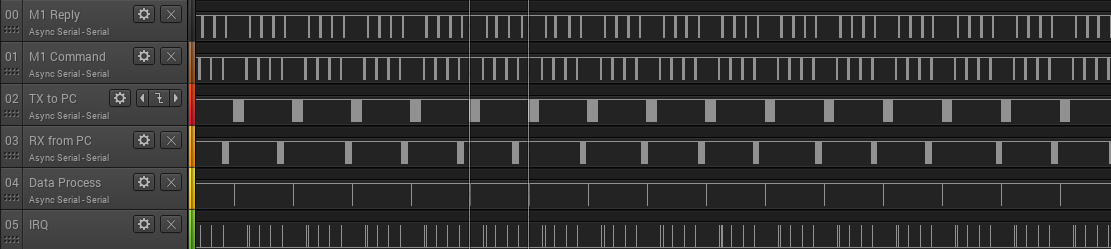
\includegraphics[width=1\textwidth]{images/comms/pc-packet-timing-data} 
\caption{Communication protocol packet timing with 5 ms sampling rate.}
\label{fig:packet-timing}
\end{figure}

\section{Graphic User Interface}
\label{chap:Graphic User Interface}

To enable rapid prototyping, a basic pre-existing serial logging platform was used and plug-ins were developed to adapt the software for controlling, configuring, logging and live plotting of the Baleka robotic leg platform. 

qSerialTerm, described as "A Qt based Serial Port terminal emulator", was built upon. It is distributed under the GNU General Public License (GPL) v3, which allows distribution, customisation and even sale of software published under the license, so long as basic conditions are met. It is copyright 2012 by Jorge Aparicio who's software repository can be found on GitHub: \url{https://github.com/JorgeAparicio/qSerialTerm}\cite{jorgeaparicio2013}.

Qt Creator CPP was used for the software development and can be compiled to run on both Linux and Windows platforms - for reference all development was completed on a Linux platform.

Three .cpp files were used for the majority of the added functionality, namely: CRC.c, framewidget.cpp and serialportwidget.cpp along with their respective header files and Qt forms.

\subsection{Serial Communication}
\label{sec:Serial Communication}

The serial interface is the first step in configuring UART communications. After successfully opening a port it allows you to select basic configuration options. The GUI extract can be seen in \cref{fig:serial-config}\cite{jorgeaparicio2013}.

A button was added, \textit{Default}, to allow quick set up of the software for experimentation with the Baleka leg. 

The maximum stable baud rate with the Qt software was 500k, any higher and the accuracy of the packet timing decreased due to application overhead. 

The refresh rate, when set to any value lower than $10\ ms$ tended to vary by as much as $5\ ms$ during operation. On Unix based operating systems the quoted accuracy of software timing is $\pm 1\ ms$ and for Windows machines it is $\pm 5\ ms$, making the decision to use a Linux machine natural. The Qt software timer resolution was increased to allow the possibility of a $200\ Hz$ refresh rate. 

The refresh rate was used to set the packet reception and transmission frequency. Due to the inconsistent timing real-time control of the leg from the Qt application was not possible, this was because of the large $\pm 60$ byte packets being transferred and the application overhead.

A compromise was found by using the Qt application for configuration of the virtual model and performing non-time critical tasks, as well as real-time logging, while the real-time control was implemented on the STM32F4 embedded system.

\begin{figure}
\centering
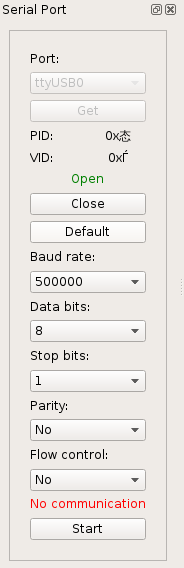
\includegraphics[width=0.2\textwidth]{images/gui/serial-port}
\caption{Serial port configuration.}
\label{fig:serial-config}
\end{figure}

\subsection{Logging and Live Plotting}

The logging software was adapted to create CSV files of all the data received from the microcontroller embedded system after it has been appropriately converted to a human readable format.

The live plotting function of the software takes an array of data of a known data size and endianness and plots the change in these values over time. There are a number of plotting options such as samples shown and format options. The live plotting proved useful for debugging of data processing issues and during experimentation to see spring-damper responses as virtual model configuration options are changed.

A number of data type conversions took place from serial reception to data plotting and logging, as follows. Qt has a number of application specific data types, usually prepended by a 'Q':

\begin{enumerate}
\item Serial data is read into the QByteArray RXBuffer.
\item RXBuffer is then copied to a char\* array to enable the packet to be decoded using the packed struct method of \cref{sec:structuring}.
\item Struct members are accessed and a union is used to convert between data types and perform calculation operations.
\item Processed data is converted to a QString using the number operator and appended to the QByteArray PlotBuffer as well as the QStringList CSVList which is converted to CSV format.
\item Finally both CSVLog and PlotBuffer are emitted as Qt signals for file logging and live plotting respectively.
\end{enumerate}

A CRC check was implemented to check the packets being received are valid. Occasionally data points are not logged or plotted - this is occasionally due to CRC failures, but usually due to the variation in processing frequency of packets due to inaccurate timing discussed in \cref{sec:Serial Communication}.

All logging and plotting development took place in the \textit{serialportwidget.cpp} file and corresponding header files and Qt forms.

The GUI for logging can be seen in \cref{fig:packet-logging} and for plotting in \cref{fig:live-plotting}.\cite{jorgeaparicio2013}

\begin{figure}
\centering
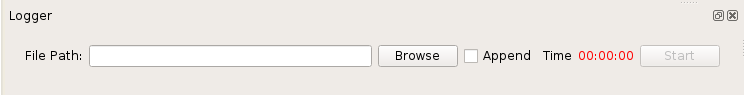
\includegraphics[width=0.5\textwidth]{images/gui/logger}
\caption{Packet data CSV logging.}
\label{fig:packet-logging}
\end{figure}

\begin{figure}
\centering
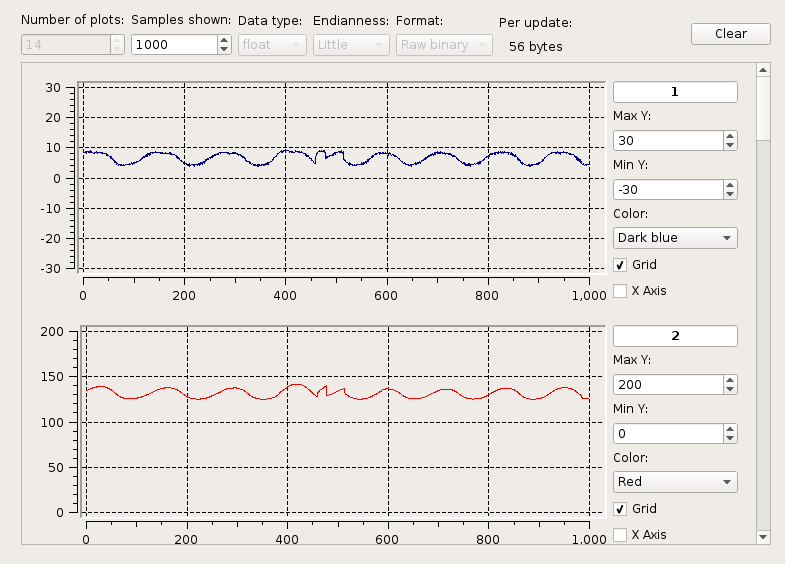
\includegraphics[width=0.5\textwidth]{images/gui/plotting}
\caption{Live plotting of motor feedback and controller data.}
\label{fig:live-plotting}
\end{figure}

\subsection{Control Plug-in}

The control plug-in was custom designed and developed for the Baleka robotic leg application. The following primary functions were integrated:

\begin{enumerate}
\item Safety.
\item Configuration.
\item Initialisation.
\item Virtual model control.
\item Sequence triggering.
\item Current and position control.
\item Control loop gain adjustment.
\end{enumerate}

The safety function of the plug-in covers not only controls to disable the motors in a case of malfunction, but also ensures that users can not enter invalid values or values that result in kinematic collisions.

The configuration and initialisation section seen in \cref{fig:Control interface plug-in} allows the motor drivers to be enabled, on-board configuration set up to be selected and the motor driver encoder position to be calibrated. 

The encoder calibration takes the current leg position and sets both $\phi_1$ and $\phi_2$ to $180^o$, measured from vertical as seen in \cref{sec:Geometry}.

The \textit{launch sequence} button combines all configuration options for a quick set up of the leg for virtual compliance or jump sequence control.

For the \textit{on-board control} and \textit{current \& position control} sections various selection boxes and text boxes exist. The underlying software ensures that, for example, current and position can not be controlled at the same time. Whenever a value changes, an update event is triggered and the data is compiled, along with an op-code, before being sent to the embedded system. The op-code then indicates to the embedded system how the data should be processed and what configuration settings should be changed.

The data processing of the control plug-in works with op-codes being added to a processing queue. When a button is pressed or a value changed, the queue is processed until empty while a switch statement based on the op-code determines where the data is placed in the packet and how it is processed. The event handlers complete the in application configuration changes.

All control plug-in functionality development took place in the \textit{framewidget.cpp} file and corresponding header files and Qt forms.

\begin{figure}
\centering
\subfloat[][Configuration \& On-board Control]{
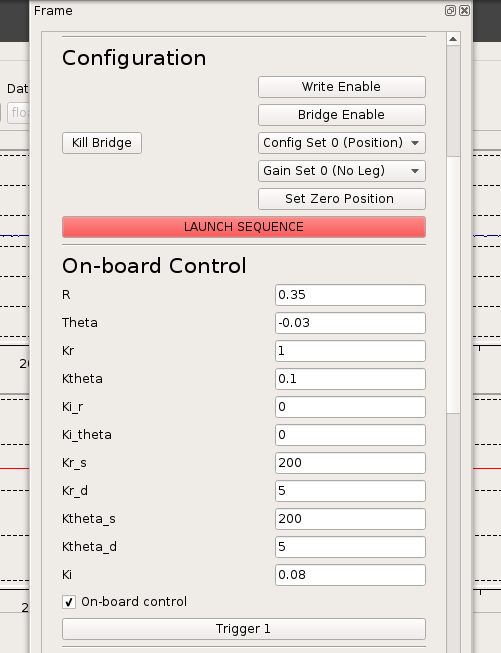
\includegraphics[width=0.4\textwidth]{images/gui/frame-1}
}
~
\subfloat[][Current/Position Control \& Control Loop Gains]{
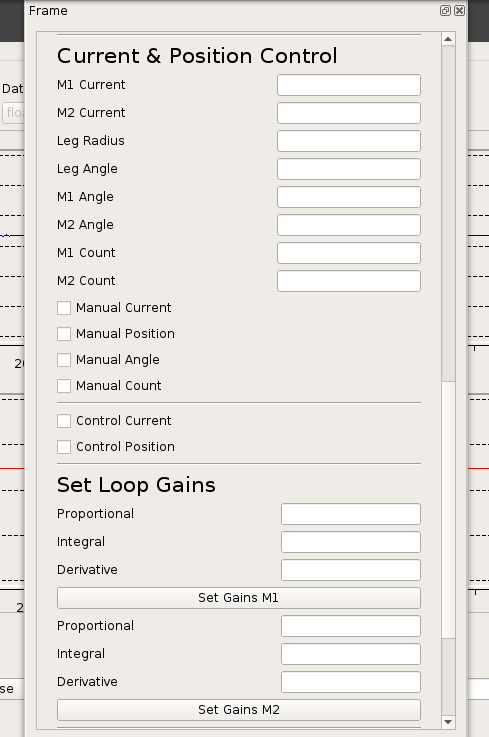
\includegraphics[width=0.4\textwidth]{images/gui/frame-2}
}
\caption{Control interface plug-in.}
\label{fig:Control interface plug-in} 
\end{figure}